\chapter{Simulation results}

In this chapter we present some selected simulations in more detail and
show some of the results\footnote{
Many more simulation results can be found at:\\
\url{http://n.ethz.ch/~raoulb/research/bachelor_thesis/simulations/}
}.

\section{The harmonic oscillator}

The harmonic oscillator is probably the most basic non-trivial potential that
fulfils the necessary smoothness assumptions. Of course we can solve this model
entirely by analytical calculations. But because of this property it's an excellent
starting point for testing and calibrating new simulation codes.

\begin{equation}
  V\ofs{x} \assign
  \begin{pmatrix}
    \frac{1}{2} \sigma x^2 & 0 \\
    0                      & \frac{1}{2} \sigma x^2
  \end{pmatrix} \quad \sigma = 0.05
\end{equation}

This potential is already diagonal, thus we can not expect any interaction of the
two components of $\Ket{\Psi}$. Figure \ref{fig:quadratic} shows the time evolution
of the energies of a wavepacket on each level. The image looks like we expected it.

\begin{figure}
  \centering
  \includegraphics[width=0.8\linewidth]{./plot/quadratic/hagedorn_energies_eigen.pdf}
  \caption{The time evolution of the energies of an initial wavepacket on each level.}
  \label{fig:quadratic}
\end{figure}

Let's now look at more interesting potentials in the next sections.

\section{A simple avoided crossing}

In this section we present some results for a potential that has a simple single
avoided crossing. We used several different values for the energy gap $\delta$.
The potential is given by the following matrix:

\begin{equation} \label{pot:delta_gap}
  V\ofs{x} \assign
  \begin{pmatrix}
    \frac{1}{2} \tanh\ofs{x} & \frac{\delta}{2} \\
    \frac{\delta}{2}         & -\frac{1}{2} \tanh\ofs{x}
  \end{pmatrix} \,.
\end{equation}

The two energy levels of this potential are

\begin{equation}
  \lambda_0 = \frac{\sqrt{{\tanh\left( x\right) }^{2}+{\delta}^{2}}}{2} \qquad
  \lambda_1 = -\frac{\sqrt{{\tanh\left(x\right) }^{2}+{\delta}^{2}}}{2}
\end{equation}

Figure \ref{fig:delta_gap} shows these two energy levels for the parameter $\delta$
set to $0.05$.

\begin{figure}
  \centering
  \includegraphics[width=0.8\linewidth]{./plot/delta_gap/potential_eigenvalues.pdf}
  \caption{Plot of the energy levels of the potential given by equation \eqref{pot:delta_gap}. The parameter $\delta$ equals $0.05$.}
  \label{fig:delta_gap}
\end{figure}

This potential is a standard example for avoided crossings and consists of nothing
but the essential properties a crossing has.

The simulation starts with an incoming Gaussian wavepacket on the upper level.
An initial momentum pointing to the right (positive $x$ axis) is used in the following.

We did several simulations within a wide range of the parameters $\varepsilon$
and $\delta$. Some of these simulations are shown here. Let's compare the operator
splitting based method with the wavepacket based one. Here we used homogeneous
wavepackets with the leading components $\chi$ set to the upper energy level.

Figures \ref{fig:delta_gap_energies_f} and \ref{fig:delta_gap_norms_f} show the
energies and the norms of $\Psi$ and it's components $\Phi_0$ on the upper level
and $\Phi_1$ on the lower one for several simulation runs based on operator
splitting. The figures \ref{fig:delta_gap_energies_h} and \ref{fig:delta_gap_norms_h}
show the simulation results obtained by using semiclassical wavepackets and identical
initial conditions. Both algorithms yield the same energy curves within the limits
of optical comparison.

From the plots of the norms we can estimate the part of the wavepacket that remains
on the respective energy level after the packet has crossed the narrow part in the
middle. While for the smallest $\delta$ most of the packet jumps over to the lower
energy level we see that for a bigger energy gap $\delta$ almost no transition
takes place.

Finally we can say that the wavepacket based algorithm works very well in this case.

\begin{figure}
  \centering
  \subfloat[][]{
    \label{fig:delta_gap_energies_f_a}
    \includegraphics[width=0.5\linewidth]{./plot/delta_gap/Parameters_f_dt0.01_eps0.1_d0.1e_p1/fourier_energies_eigen.pdf}
  }
  \subfloat[][]{
    \label{fig:delta_gap_energies_f_b}
    \includegraphics[width=0.5\linewidth]{./plot/delta_gap/Parameters_f_dt0.01_eps0.1_d0.5e_p1/fourier_energies_eigen.pdf}
  } \\
  \subfloat[][]{
    \label{fig:delta_gap_energies_f_c}
    \includegraphics[width=0.5\linewidth]{./plot/delta_gap/Parameters_f_dt0.01_eps0.1_d1.0e_p1/fourier_energies_eigen.pdf}
  }
  \subfloat[][]{
    \label{fig:delta_gap_energies_f_d}
    \includegraphics[width=0.5\linewidth]{./plot/delta_gap/Parameters_f_dt0.01_eps0.1_d1.5e_p1/fourier_energies_eigen.pdf}
  } \\
  \subfloat[][]{
    \label{fig:delta_gap_energies_f_e}
    \includegraphics[width=0.5\linewidth]{./plot/delta_gap/Parameters_f_dt0.01_eps0.1_d2.0e_p1/fourier_energies_eigen.pdf}
  }
  \subfloat[][]{
    \label{fig:legend_energies_2}
    \includegraphics[scale=0.3]{./plot/legend_energies_2.png}
  } \\
  \caption[Plots of the energies of the wavepacket's individual components $\Phi_i$.]{
    Plots of the energies of the wavepacket's individual components $\Phi_i$. These
    results were obtained by the operator splitting method.
    \subref{fig:delta_gap_energies_f_a} $\varepsilon = 0.1$ and $\delta = 0.1 \varepsilon$
    \subref{fig:delta_gap_energies_f_b} $\varepsilon = 0.1$ and $\delta = 0.5 \varepsilon$
    \subref{fig:delta_gap_energies_f_c} $\varepsilon = 0.1$ and $\delta = 1.0 \varepsilon$
    \subref{fig:delta_gap_energies_f_d} $\varepsilon = 0.1$ and $\delta = 1.5 \varepsilon$
    \subref{fig:delta_gap_energies_f_e} $\varepsilon = 0.1$ and $\delta = 2.0 \varepsilon$
    \label{fig:delta_gap_energies_f}
  }
\end{figure}

\begin{figure}
  \centering
  \subfloat[][]{
    \label{fig:delta_gap_norms_f_a}
    \includegraphics[width=0.5\linewidth]{./plot/delta_gap/Parameters_f_dt0.01_eps0.1_d0.1e_p1/fourier_norms_eigen.pdf}
  }
  \subfloat[][]{
    \label{fig:delta_gap_norms_f_b}
    \includegraphics[width=0.5\linewidth]{./plot/delta_gap/Parameters_f_dt0.01_eps0.1_d0.5e_p1/fourier_norms_eigen.pdf}
  } \\
  \subfloat[][]{
    \label{fig:delta_gap_norms_f_c}
    \includegraphics[width=0.5\linewidth]{./plot/delta_gap/Parameters_f_dt0.01_eps0.1_d1.0e_p1/fourier_norms_eigen.pdf}
  }
  \subfloat[][]{
    \label{fig:delta_gap_norms_f_d}
    \includegraphics[width=0.5\linewidth]{./plot/delta_gap/Parameters_f_dt0.01_eps0.1_d1.5e_p1/fourier_norms_eigen.pdf}
  } \\
  \subfloat[][]{
    \label{fig:delta_gap_norms_f_e}
    \includegraphics[width=0.5\linewidth]{./plot/delta_gap/Parameters_f_dt0.01_eps0.1_d2.0e_p1/fourier_norms_eigen.pdf}
  }
  \subfloat[][]{
    \label{fig:legend_norms_2}
    \includegraphics[scale=0.3]{./plot/legend_norms_2.png}
  } \\

  \caption[Plots of the norms of the wavepacket's individual components $\Phi_i$]{
    Plots of the norms of the wavepacket's individual components $\Phi_i$. These
    results were obtained by the operator splitting method.
    \subref{fig:delta_gap_norms_f_a} $\varepsilon = 0.1$ and $\delta = 0.1 \varepsilon$
    \subref{fig:delta_gap_norms_f_b} $\varepsilon = 0.1$ and $\delta = 0.5 \varepsilon$
    \subref{fig:delta_gap_norms_f_c} $\varepsilon = 0.1$ and $\delta = 1.0 \varepsilon$
    \subref{fig:delta_gap_norms_f_d} $\varepsilon = 0.1$ and $\delta = 1.5 \varepsilon$
    \subref{fig:delta_gap_norms_f_e} $\varepsilon = 0.1$ and $\delta = 2.0 \varepsilon$
    \label{fig:delta_gap_norms_f}
  }
\end{figure}

\begin{figure}
  \centering
  \subfloat[][]{
    \label{fig:delta_gap_energies_h_a}
    \includegraphics[width=0.5\linewidth]{./plot/delta_gap/Parameters_h_dt0.01_eps0.1_d0.1e_p1/hagedorn_energies_eigen.pdf}
  }
  \subfloat[][]{
    \label{fig:delta_gap_energies_h_b}
    \includegraphics[width=0.5\linewidth]{./plot/delta_gap/Parameters_h_dt0.01_eps0.1_d0.5e_p1/hagedorn_energies_eigen.pdf}
  } \\
  \subfloat[][]{
    \label{fig:delta_gap_energies_h_c}
    \includegraphics[width=0.5\linewidth]{./plot/delta_gap/Parameters_h_dt0.01_eps0.1_d1.0e_p1/hagedorn_energies_eigen.pdf}
  }
  \subfloat[][]{
    \label{fig:delta_gap_energies_h_d}
    \includegraphics[width=0.5\linewidth]{./plot/delta_gap/Parameters_h_dt0.01_eps0.1_d1.5e_p1/hagedorn_energies_eigen.pdf}
  } \\
  \subfloat[][]{
    \label{fig:delta_gap_energies_h_e}
    \includegraphics[width=0.5\linewidth]{./plot/delta_gap/Parameters_h_dt0.01_eps0.1_d2.0e_p1/hagedorn_energies_eigen.pdf}
  }
  \subfloat[][]{
    \includegraphics[scale=0.3]{./plot/legend_energies_2.png}
  } \\
  \caption[Plots of the energies of the wavepacket's individual components $\Phi_i$.]{
    Plots of the energies of the wavepacket's individual components $\Phi_i$. These
    results were obtained by propagating wavepackets.
    \subref{fig:delta_gap_energies_h_a} $\varepsilon = 0.1$ and $\delta = 0.1 \varepsilon$
    \subref{fig:delta_gap_energies_h_b} $\varepsilon = 0.1$ and $\delta = 0.5 \varepsilon$
    \subref{fig:delta_gap_energies_h_c} $\varepsilon = 0.1$ and $\delta = 1.0 \varepsilon$
    \subref{fig:delta_gap_energies_h_d} $\varepsilon = 0.1$ and $\delta = 1.5 \varepsilon$
    \subref{fig:delta_gap_energies_h_e} $\varepsilon = 0.1$ and $\delta = 2.0 \varepsilon$
    \label{fig:delta_gap_energies_h}
  }
\end{figure}

\begin{figure}
  \centering
  \subfloat[][]{
    \label{fig:delta_gap_norms_h_a}
    \includegraphics[width=0.5\linewidth]{./plot/delta_gap/Parameters_h_dt0.01_eps0.1_d0.1e_p1/hagedorn_norms_eigen.pdf}
  }
  \subfloat[][]{
    \label{fig:delta_gap_norms_h_b}
    \includegraphics[width=0.5\linewidth]{./plot/delta_gap/Parameters_h_dt0.01_eps0.1_d0.5e_p1/hagedorn_norms_eigen.pdf}
  } \\
  \subfloat[][]{
    \label{fig:delta_gap_norms_h_c}
    \includegraphics[width=0.5\linewidth]{./plot/delta_gap/Parameters_h_dt0.01_eps0.1_d1.0e_p1/hagedorn_norms_eigen.pdf}
  }
  \subfloat[][]{
    \label{fig:delta_gap_norms_h_d}
    \includegraphics[width=0.5\linewidth]{./plot/delta_gap/Parameters_h_dt0.01_eps0.1_d1.5e_p1/hagedorn_norms_eigen.pdf}
  } \\
  \subfloat[][]{
    \label{fig:delta_gap_norms_h_e}
    \includegraphics[width=0.5\linewidth]{./plot/delta_gap/Parameters_h_dt0.01_eps0.1_d2.0e_p1/hagedorn_norms_eigen.pdf}
  }
  \subfloat[][]{
    \includegraphics[scale=0.3]{./plot/legend_norms_2.png}
  } \\

  \caption[Plots of the norms of the wavepacket's individual components $\Phi_i$]{
    Plots of the norms of the wavepacket's individual components $\Phi_i$. These
    results were obtained by propagating wavepackets.
    \subref{fig:delta_gap_norms_h_a} $\varepsilon = 0.1$ and $\delta = 0.1 \varepsilon$
    \subref{fig:delta_gap_norms_h_b} $\varepsilon = 0.1$ and $\delta = 0.5 \varepsilon$
    \subref{fig:delta_gap_norms_h_c} $\varepsilon = 0.1$ and $\delta = 1.0 \varepsilon$
    \subref{fig:delta_gap_norms_h_d} $\varepsilon = 0.1$ and $\delta = 1.5 \varepsilon$
    \subref{fig:delta_gap_norms_h_e} $\varepsilon = 0.1$ and $\delta = 2.0 \varepsilon$
    \label{fig:delta_gap_norms_h}
  }
\end{figure}

It may be interesting to see the time evolution of the Hagedorn parameters $\Pi$
and the coefficients $c^i$ of a wavepacket $\Ket{\Psi}$. In the figure \ref{fig:delta_gap_hagedorn_params_evolution}
we see the evolution of the parameters. The figures \ref{fig:delta_gap_coefficients_first}
and \ref{fig:delta_gap_coefficients_last}
show the first and last four coefficients of both components $\Phi_i$. The general
setup of the simulation corresponds to the example in the above figures \ref{fig:delta_gap_energies_h_c}
and \ref{fig:delta_gap_norms_h_c}

\begin{figure}
  \centering
  \includegraphics[width=\linewidth]{./plot/delta_gap/Parameters_h_dt0.01_eps0.1_d1.0e_p1/hagedorn_parameters.pdf}
  \caption{Plot of the time evolution of the Hagedorn parameters $P$, $Q$, $S$, $p$ and $q$. Mind the scales!}
  \label{fig:delta_gap_hagedorn_params_evolution}
\end{figure}

\begin{figure}
  \centering
  \includegraphics[width=\linewidth]{./plot/delta_gap/Parameters_h_dt0.01_eps0.1_d1.0e_p1/hagedorn_coefficients_first.pdf}
  \caption{Plot of the time evolution of the first 4 coefficients $c_0$, $c_1$, $c_2$, $c_3$ for both components. The blue and the green line are the
  real and the imaginary part, and the red one is the absolute value. Mind the scales!}
  \label{fig:delta_gap_coefficients_first}
\end{figure}

\begin{figure}
  \centering
  \includegraphics[width=\linewidth]{./plot/delta_gap/Parameters_h_dt0.01_eps0.1_d1.0e_p1/hagedorn_coefficients_last.pdf}
  \caption{Plot of the time evolution of the last 4 coefficients $c_{-4}$, $c_{-3}$, $c_{-2}$, $c_{-1}$ for both components. The blue and the green line are the
  real and the imaginary part, and the red one is the absolute value. Mind the scales!}
  \label{fig:delta_gap_coefficients_last}
\end{figure}


\section{Two avoided crossings in series}
\label{sec:two_crossings}

After we have seen the simulation results for a single avoided crossing let's look at
another interesting question. That is, what happens if we have multiple of these
avoided crossings in series. When entering the second one, the wavepacket is
already scattered to both energy levels. But first we define the potential:

\begin{equation} \label{pot:two_crossings}
  V\ofs{x} \assign
  \begin{pmatrix}
    \frac{1}{2} \tanh\ofs{x-\sigma} \tanh\ofs{x+\sigma} & \frac{\delta}{2} \\
    \frac{\delta}{2}                                    & -\frac{1}{2} \tanh\ofs{x-\sigma} \tanh\ofs{x+\sigma}
  \end{pmatrix} \quad \sigma = 3 \,.
\end{equation}

The parameter $\sigma$ determines the location of the avoided crossings. For an
even longer series we could use a product of more factors:

\begin{equation}
  V_{0,0}\ofs{x} \assign \prod_i \tanh\ofs{x-\sigma_i}
\end{equation}

for an arbitrary set $\{\sigma_i\}_i$ and $V_{1,1} \assign -V_{0,0}$. However
let's return to the simplest case of only two narrow parts. The two energy levels
of this potential are given by:

\begin{equation}
  \lambda = \pm \frac{\sqrt{{\tanh\left( x-\sigma\right) }^{2}\,{\tanh\left( x+\sigma\right) }^{2}+{\delta}^{2}}}{2} \,.
\end{equation}

Figure \ref{fig:two_crossings} shows these two energy levels for the parameter $\delta$
set to $0.05$. The effect of the parameter $\delta$ is shown in the plot \ref{fig:two_crossings_multi}
for multiple values ranging from $0.5 \varepsilon$ up to $10 \varepsilon$. For
bigger $\delta$ we get an increasing energy gap and also much smoother insections.

\begin{figure}
  \centering
  \includegraphics[width=0.8\linewidth]{./plot/two_crossings/potential_eigenvalues.pdf}
  \caption{Plot of the energy levels of the potential given by equation \eqref{pot:two_crossings}. The parameter $\delta$ equals $0.05$.}
  \label{fig:two_crossings}
\end{figure}

\begin{figure}
  \centering
  \includegraphics[width=0.8\linewidth]{./plot/two_crossings/potential_eigenvalues_multi2.pdf}
  \caption{The effect of the parameter $\delta$ on the energy levels.}
  \label{fig:two_crossings_multi}
\end{figure}

The figures in \ref{fig:two_crossings_energies_f} show the energy evolution of a wavepacket
traversing the potential shown in \ref{fig:two_crossings}. The norms of the individual
components are shown on figure \ref{fig:two_crossings_norms_f} and we can see how most of the
packet jumps over to the lower level at the first crossing and back to the upper at
the second one. For big $\delta$ the packet does almost not react to the lower level's bumps.
These results were obtained by the operator splitting ansatz which works very well here.

\begin{figure}
  \centering
  \subfloat[][]{
    \label{fig:two_crossings_energies_f_a}
    \includegraphics[width=0.5\linewidth]{./plot/two_crossings/Parameters_f_dt0.02_eps0.2_d0.5e_p1/fourier_energies_eigen.pdf}
  }
  \subfloat[][]{
    \label{fig:two_crossings_energies_f_b}
    \includegraphics[width=0.5\linewidth]{./plot/two_crossings/Parameters_f_dt0.02_eps0.2_d1.0e_p1/fourier_energies_eigen.pdf}
  } \\
  \subfloat[][]{
    \label{fig:two_crossings_energies_f_c}
    \includegraphics[width=0.5\linewidth]{./plot/two_crossings/Parameters_f_dt0.02_eps0.2_d1.5e_p1/fourier_energies_eigen.pdf}
  }
  \subfloat[][]{
    \label{fig:two_crossings_energies_f_d}
    \includegraphics[width=0.5\linewidth]{./plot/two_crossings/Parameters_f_dt0.02_eps0.2_d2.0e_p1/fourier_energies_eigen.pdf}
  } \\
  \subfloat[][]{
    \label{fig:two_crossings_energies_f_e}
    \includegraphics[width=0.5\linewidth]{./plot/two_crossings/Parameters_f_dt0.02_eps0.2_d2.5e_p1/fourier_energies_eigen.pdf}
  }
  \subfloat[][]{
    \label{fig:two_crossings_energies_f_f}
    \includegraphics[width=0.5\linewidth]{./plot/two_crossings/Parameters_f_dt0.02_eps0.2_d4.0e_p1/fourier_energies_eigen.pdf}
  } \\
  \caption[Plots of the energies of the wavepacket's individual components $\Phi_i$.]{
    Plots of the energies of the wavepacket's individual components $\Phi_i$. These
    results were obtained by the operator splitting method. (The legend for these figures
    is shown in \ref{fig:legend_energies_2})
    \subref{fig:two_crossings_energies_f_a} $\varepsilon = 0.2$ and $\delta = 0.5 \varepsilon$
    \subref{fig:two_crossings_energies_f_b} $\varepsilon = 0.2$ and $\delta = 1.0 \varepsilon$
    \subref{fig:two_crossings_energies_f_c} $\varepsilon = 0.2$ and $\delta = 1.5 \varepsilon$
    \subref{fig:two_crossings_energies_f_d} $\varepsilon = 0.2$ and $\delta = 2.0 \varepsilon$
    \subref{fig:two_crossings_energies_f_e} $\varepsilon = 0.2$ and $\delta = 2.5 \varepsilon$
    \subref{fig:two_crossings_energies_f_f} $\varepsilon = 0.2$ and $\delta = 4.0 \varepsilon$
    \label{fig:two_crossings_energies_f}
  }
\end{figure}

\begin{figure}
  \centering
  \subfloat[][]{
    \label{fig:two_crossings_norms_f_a}
    \includegraphics[width=0.5\linewidth]{./plot/two_crossings/Parameters_f_dt0.02_eps0.2_d0.5e_p1/fourier_norms_eigen.pdf}
  }
  \subfloat[][]{
    \label{fig:two_crossings_norms_f_b}
    \includegraphics[width=0.5\linewidth]{./plot/two_crossings/Parameters_f_dt0.02_eps0.2_d1.0e_p1/fourier_norms_eigen.pdf}
  } \\
  \subfloat[][]{
    \label{fig:two_crossings_norms_f_c}
    \includegraphics[width=0.5\linewidth]{./plot/two_crossings/Parameters_f_dt0.02_eps0.2_d1.5e_p1/fourier_norms_eigen.pdf}
  }
  \subfloat[][]{
    \label{fig:two_crossings_norms_f_d}
    \includegraphics[width=0.5\linewidth]{./plot/two_crossings/Parameters_f_dt0.02_eps0.2_d2.0e_p1/fourier_norms_eigen.pdf}
  } \\
  \subfloat[][]{
    \label{fig:two_crossings_norms_f_e}
    \includegraphics[width=0.5\linewidth]{./plot/two_crossings/Parameters_f_dt0.02_eps0.2_d2.5e_p1/fourier_norms_eigen.pdf}
  }
  \subfloat[][]{
    \label{fig:two_crossings_norms_f_f}
    \includegraphics[width=0.5\linewidth]{./plot/two_crossings/Parameters_f_dt0.02_eps0.2_d4.0e_p1/fourier_norms_eigen.pdf}
  } \\
  \caption[Plots of the norms of the wavepacket's individual components $\Phi_i$.]{
    Plots of the norms of the wavepacket's individual components $\Phi_i$. These
    results were obtained by the operator splitting method. (The legend for these figures
    is shown in \ref{fig:legend_norms_2})
    \subref{fig:two_crossings_norms_f_a} $\varepsilon = 0.2$ and $\delta = 0.5 \varepsilon$
    \subref{fig:two_crossings_norms_f_b} $\varepsilon = 0.2$ and $\delta = 1.0 \varepsilon$
    \subref{fig:two_crossings_norms_f_c} $\varepsilon = 0.2$ and $\delta = 1.5 \varepsilon$
    \subref{fig:two_crossings_norms_f_d} $\varepsilon = 0.2$ and $\delta = 2.0 \varepsilon$
    \subref{fig:two_crossings_norms_f_e} $\varepsilon = 0.2$ and $\delta = 2.5 \varepsilon$
    \subref{fig:two_crossings_norms_f_f} $\varepsilon = 0.2$ and $\delta = 4.0 \varepsilon$
    \label{fig:two_crossings_norms_f}
  }
\end{figure}

For this potential the wavepacket based algorithm breaks down as soon as the packet
arrives at the second crossing for yet unknown reasons. This is true at least for small values
of $\delta$. For big $\delta$ the time evolution gets better and better.
But we can not resolve the interesting details for small $\varepsilon$ and $\delta$.
We used a basis of size $K=64$. One might think that the basis is just too small
but other tests with $K = 128$ and even $K = 256$ showed the same issues. The algorithm
broke down just a few timesteps later. Hence we can conclude that the algorithm does
not work in this configuration for yet unknown reasons.

\begin{figure}
  \centering
  \subfloat[][]{
    \label{fig:two_crossings_energies_h_a}
    \includegraphics[width=0.5\linewidth]{./plot/two_crossings/Parameters_h_dt0.02_eps0.2_d0.5e_p1/hagedorn_energies_eigen.pdf}
  }
  \subfloat[][]{
    \label{fig:two_crossings_energies_h_b}
    \includegraphics[width=0.5\linewidth]{./plot/two_crossings/Parameters_h_dt0.02_eps0.2_d1.0e_p1/hagedorn_energies_eigen.pdf}
  } \\
  \subfloat[][]{
    \label{fig:two_crossings_energies_h_c}
    \includegraphics[width=0.5\linewidth]{./plot/two_crossings/Parameters_h_dt0.02_eps0.2_d1.5e_p1/hagedorn_energies_eigen.pdf}
  }
  \subfloat[][]{
    \label{fig:two_crossings_energies_h_d}
    \includegraphics[width=0.5\linewidth]{./plot/two_crossings/Parameters_h_dt0.02_eps0.2_d2.0e_p1/hagedorn_energies_eigen.pdf}
  } \\
  \subfloat[][]{
    \label{fig:two_crossings_energies_h_e}
    \includegraphics[width=0.5\linewidth]{./plot/two_crossings/Parameters_h_dt0.02_eps0.2_d2.5e_p1/hagedorn_energies_eigen.pdf}
  }
  \subfloat[][]{
    \label{fig:two_crossings_energies_h_f}
    \includegraphics[width=0.5\linewidth]{./plot/two_crossings/Parameters_h_dt0.02_eps0.2_d4.0e_p1/hagedorn_energies_eigen.pdf}
  } \\
  \caption[Plots of the energies of the wavepacket's individual components $\Phi_i$.]{
    Plots of the energies of the wavepacket's individual components $\Phi_i$. These
    results were obtained by propagating wavepackets. (The legend for these figures
    is shown in \ref{fig:legend_energies_2})
    \subref{fig:two_crossings_energies_h_a} $\varepsilon = 0.2$ and $\delta = 0.5 \varepsilon$
    \subref{fig:two_crossings_energies_h_b} $\varepsilon = 0.2$ and $\delta = 1.0 \varepsilon$
    \subref{fig:two_crossings_energies_h_c} $\varepsilon = 0.2$ and $\delta = 1.5 \varepsilon$
    \subref{fig:two_crossings_energies_h_d} $\varepsilon = 0.2$ and $\delta = 2.0 \varepsilon$
    \subref{fig:two_crossings_energies_h_e} $\varepsilon = 0.2$ and $\delta = 2.5 \varepsilon$
    \subref{fig:two_crossings_energies_h_f} $\varepsilon = 0.2$ and $\delta = 4.0 \varepsilon$
    \label{fig:two_crossings_energies_h}
  }
\end{figure}


\section{A potential with three energy levels}

Finally we want to look at a potential with three energy levels. This also tests
the numerical abilities of our code as we can not do analytical calculations for
this matrix and the implementation falls back to pure numerical algorithms. First
of all, this is the matrix we use:

\begin{equation} \label{pot:three_states}
  V\ofs{x} \assign
  \begin{pmatrix}
    \tanh\ofs{x+\sigma} + \tanh\ofs{x-\sigma} & \delta_1             & \delta_2 \\
    \delta_1                                  & -\tanh\ofs{x+\sigma} & 0 \\
    \delta_2                                  & 0                    & 1-\tanh\ofs{x-\sigma}
  \end{pmatrix} \,.
\end{equation}

For this potential we can no longer give an analytical closed form expression
for the eigenvalues. Hence we use numerical eigenvalue calculation. The procedure
is very similar to what we sketched in figure \ref{fig:matrix_exponential_num}.
Figure \ref{fig:three_states} shows all three energy levels $\lambda_0\ofs{x}$, $\lambda_1\ofs{x}$, $\lambda_2\ofs{x}$
for the parameters $\delta_1 = \delta_2 = \delta$ set to $0.05$.

\begin{figure}
  \centering
  \includegraphics[width=0.8\linewidth]{./plot/three_states/potential_eigenvalues.pdf}
  \caption{Plot of the energy levels of the potential given by equation \eqref{pot:three_states}.
  The parameters $\delta_i$ equal $0.05$.}
  \label{fig:three_states}
\end{figure}

In this asymmetric energy landscape we expect a rich set of different transitions
between all levels. Figure \ref{fig:three_states_energies} shows the energy curves
for a Gaussian wavepacket in different initial situations entering the potential
from the left or the right. The simulations are all done with the operator splitting
method. A reason for this is that the wavepackets break down already for the much
simpler case presented in \ref{fig:two_crossings_energies_h}.

\begin{figure}
  \centering
  \subfloat[][]{
    \includegraphics[scale=0.3]{./plot/legend_energies_3.png}
    \label{fig:legend_energies_3}
  }
  \subfloat[][]{
    \includegraphics[scale=0.3]{./plot/legend_norms_3.png}
    \label{fig:legend_norms_3}
  } \\
  \caption[Legends]{
    Legends of the figures \ref{fig:three_states_energies} and \ref{fig:three_states_norms}.
  }
\end{figure}

\begin{figure}
  \centering
  \subfloat[][]{
    \label{fig:three_states_energies_a}
    \includegraphics[width=0.5\linewidth]{./plot/three_states/Parameters_f_l_0/fourier_energies_eigen.pdf}
  }
  \subfloat[][]{
    \label{fig:three_states_energies_b}
    \includegraphics[width=0.5\linewidth]{./plot/three_states/Parameters_f_r_0/fourier_energies_eigen.pdf}
  } \\
  \subfloat[][]{
    \label{fig:three_states_energies_c}
    \includegraphics[width=0.5\linewidth]{./plot/three_states/Parameters_f_l_1/fourier_energies_eigen.pdf}
  }
  \subfloat[][]{
    \label{fig:three_states_energies_d}
    \includegraphics[width=0.5\linewidth]{./plot/three_states/Parameters_f_r_1/fourier_energies_eigen.pdf}
  } \\
  \subfloat[][]{
    \label{fig:three_states_energies_e}
    \includegraphics[width=0.5\linewidth]{./plot/three_states/Parameters_f_l_2/fourier_energies_eigen.pdf}
  }
  \subfloat[][]{
    \label{fig:three_states_energies_f}
    \includegraphics[width=0.5\linewidth]{./plot/three_states/Parameters_f_r_2/fourier_energies_eigen.pdf}
  } \\
  \caption[Plots of the energies of the wavepacket's individual components $\Phi_i$.]{
    Plots of the energies of the wavepacket's individual components $\Phi_i$. (The legend for these figure
    is shown in \ref{fig:legend_energies_3})
    \subref{fig:three_states_energies_a} A wavepacket $\Ket{\Psi}$ on the upper most level coming from the left.
    \subref{fig:three_states_energies_b} A wavepacket $\Ket{\Psi}$ on the upper most level coming from the right.
    \subref{fig:three_states_energies_c} A wavepacket $\Ket{\Psi}$ on the middle level coming from the left.
    \subref{fig:three_states_energies_d} A wavepacket $\Ket{\Psi}$ on the middle level coming from the right.
    \subref{fig:three_states_energies_e} A wavepacket $\Ket{\Psi}$ on the lowest level coming from the left.
    \subref{fig:three_states_energies_f} A wavepacket $\Ket{\Psi}$ on the lowest level coming from the right.
    \label{fig:three_states_energies}
  }
\end{figure}

The figures in table \ref{fig:three_states_norms} show the evolution of the norms
of all components $\Phi_i$ of $\Ket{\Psi}$. From these plots we can estimate the
transitions that take place. The plots correspond to the ones in figure \ref{fig:three_states_energies}.

\begin{figure}
  \centering
  \subfloat[][]{
    \label{fig:three_states_norms_a}
    \includegraphics[width=0.5\linewidth]{./plot/three_states/Parameters_f_l_0/fourier_norms_eigen.pdf}
  }
  \subfloat[][]{
    \label{fig:three_states_norms_b}
    \includegraphics[width=0.5\linewidth]{./plot/three_states/Parameters_f_r_0/fourier_norms_eigen.pdf}
  } \\
  \subfloat[][]{
    \label{fig:three_states_norms_c}
    \includegraphics[width=0.5\linewidth]{./plot/three_states/Parameters_f_l_1/fourier_norms_eigen.pdf}
  }
  \subfloat[][]{
    \label{fig:three_states_norms_d}
    \includegraphics[width=0.5\linewidth]{./plot/three_states/Parameters_f_r_1/fourier_norms_eigen.pdf}
  } \\
  \subfloat[][]{
    \label{fig:three_states_norms_e}
    \includegraphics[width=0.5\linewidth]{./plot/three_states/Parameters_f_l_2/fourier_norms_eigen.pdf}
  }
  \subfloat[][]{
    \label{fig:three_states_norms_f}
    \includegraphics[width=0.5\linewidth]{./plot/three_states/Parameters_f_r_2/fourier_norms_eigen.pdf}
  } \\
  \caption[Plots of the norms of the wavepacket's individual components $\Phi_i$.]{
    Plots of the norms of the wavepacket's individual components $\Phi_i$. (The legend for these figure
    is shown in \ref{fig:legend_norms_3})
    \subref{fig:three_states_norms_a} A wavepacket $\Ket{\Psi}$ on the upper most level coming from the left.
    \subref{fig:three_states_norms_b} A wavepacket $\Ket{\Psi}$ on the upper most level coming from the right.
    \subref{fig:three_states_norms_c} A wavepacket $\Ket{\Psi}$ on the middle level coming from the left.
    \subref{fig:three_states_norms_d} A wavepacket $\Ket{\Psi}$ on the middle level coming from the right.
    \subref{fig:three_states_norms_e} A wavepacket $\Ket{\Psi}$ on the lowest level coming from the left.
    \subref{fig:three_states_norms_f} A wavepacket $\Ket{\Psi}$ on the lowest level coming from the right.
    \label{fig:three_states_norms}
  }
\end{figure}
